\section{21 - MAT - AG 2.1, AN 1.3, AN 2.1, FA 1.7 - Blutgefäß - BIFIE Aufgabensammlung}

\begin{langesbeispiel} \item[0] %PUNKTE DES BEISPIELS
				In einem Blutgefäß hingt die Geschwindigkeit $v$ des Blutes davon ab, wie groß der Abstand $x$ zum Mittelpunkt ist. ein gültiger Zusammenhang zwischen der Geschwindigkeit $v$ und dem Abstand $x$ kann mittels einer Formel $v(x)=v_m\cdot (1-\frac{x^2}{R^2})$ modelliert werden.
				
				\begin{center}\resizebox{0.8\linewidth}{!}{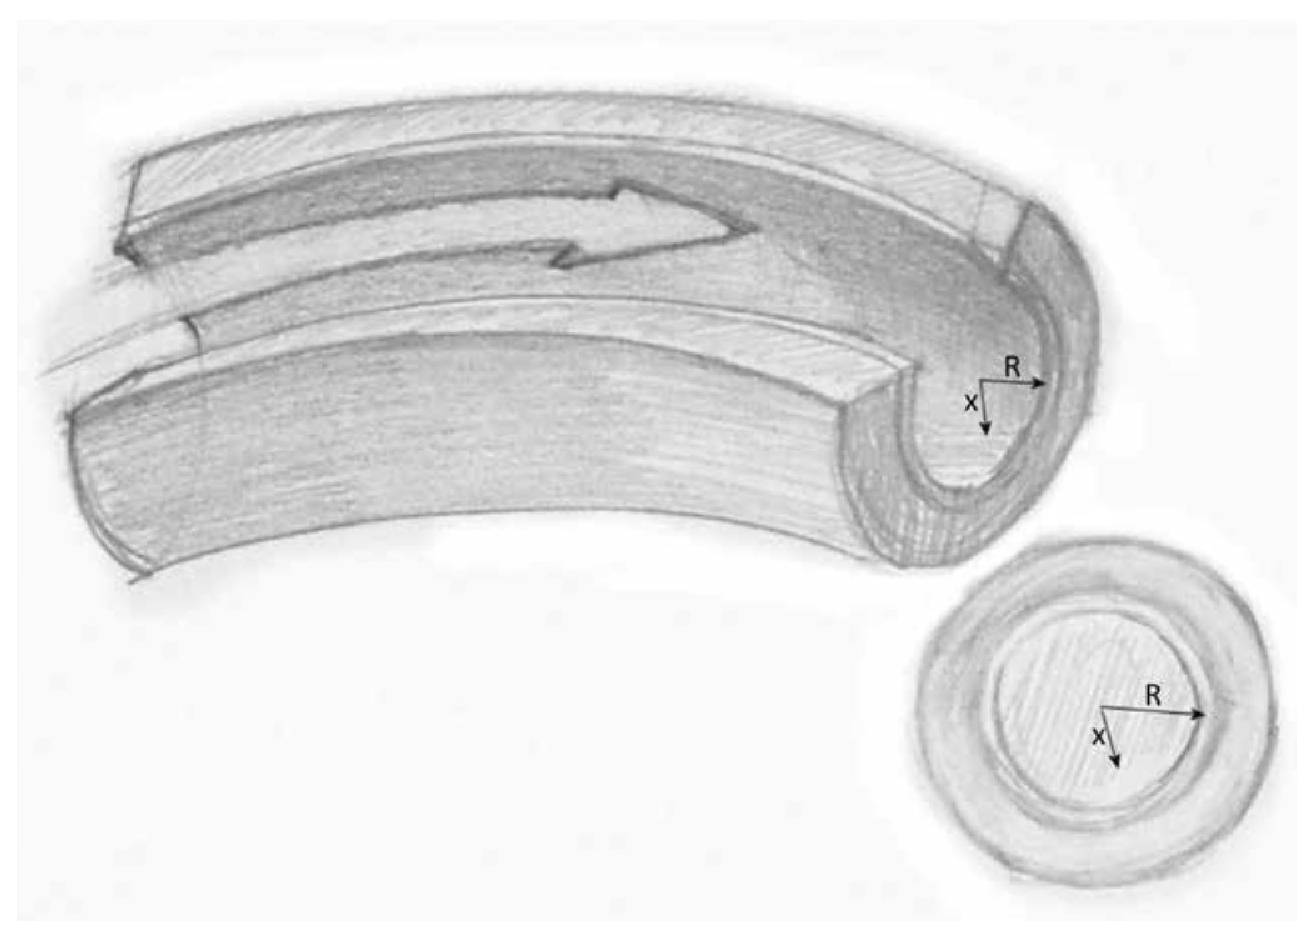
\includegraphics{../_database/Bilder/Bild21-1.eps}}\end{center}
				
				\begin{singlespace}
\begin{tiny}
(Quelle: http://www.gefaesschirurgie
-klinik.de/patienteninformationen/arterienverkalkung.php, ergänzt durch Pfeile und Beschriftung) 
\end{tiny}
\end{singlespace}

Die in der Formel auftretenden Größen sind im Foglenden beschrieben:\leer

$R$ ... Innenradius des Blutgefäßes in mm

$v_m$ ... maximale Geschwindigkeit des Blutes im Mittelpunkt des Blutgefäßes in cm/s

$x$ ... Abstand vom Mittelpunkt des Blutgefäßes in mm

$v(x)$ ... Geschwindigkeit des Blutes bei Abstand $x$ vom Mittelpunkt des Blutgefäßes in cm/s

\subsection{Aufgabenstellung:}
\begin{enumerate}
	\item Gib einen Definitionsbereich für $x$ an, der für das Blutgefäß sinnvoll ist, und begründe, warum die Formel eine vereinfachte Beschreibung der Blutgeschwindigkeit ist!
	
	\item In einem Lehrbuch der Medizin wird bhauptet, dass beim Abstand $x=\frac{R}{2}$ die Geschwindigkeit des Blutes $75\,\%$ vom maximalen Wert beträgt. Um diese Aussage mathematisch zu beweisen, wird der Ansatz $v(x)=\frac{3}{4}\,v_m$ gemacht, und damit wird die Stelle $x$ berechnet.
	
	Führe die Berechnung von der Stelle $x$ aus und zeige, dass man mit der Berechnung des Funktionswertes $v\left\langle \frac{R}{2}\right\rangle$ zum gleichen Ergebnis kommt!
	
	\item Forme die gegebene Formel für $v(x)$ so um, dass man eine Funktion $x(v)$ erhält!
	
	Erläutere, was der Funktionswert $x\left(\frac{v_m}{2}\right)$ für die Blutströmung bedeutet!
	
	\item Gib die momentane Änderungsrate der Geschwindigkeit $v$ (bei Veränderung von $x$) beim Abstand $x$ an und gib an, was das Vorzeichen der Änderungsrate über das Verhalten der Blutströmung aussagt!
	
						\end{enumerate}\leer
				
\antwort{\subsection{Lösungserwartung:}
\begin{enumerate}
	\item Der Definitionsbereich ist $[0;R]$ (Minimalanforderung: Angabe des Intervalls).
	
	Negative Abstände $(x<0)$ sind sinnlos, und $x>R$ würde bedeuten, dass das Blutkörperchen außerhalb des Blutgefäßes ist.\leer
	
	Die Formel ist deswegen eine Vereinfachung, weil das Blut am Innenrand des Blutgefäßes bestimmt nicht die Geschwindigkeit 0 hat. 
	
	Außerdem setzt die Formel voraus, dass das Blutgefäß an jeder Stelle einen kreisförmigen Querschnitt mit einem konstanten Radius $R$ hat bzw. dass das Blutgefäß exakt zylinderförmig ist (Venen haben auch Venenklappen).
	
Schließlich strömt das Blut zeitlich nicht mit konstanter Geschwindigkeit,
 die Blutgeschwindigkeit verändert sich periodisch.

\item Lösungsweg 1:

Umformen: $\frac{3}{4}v_m=v_m\cdot\left(1-\frac{x^2}{R^2}\right)\Rightarrow\frac{3}{4}=1-\frac{x^2}{R^2}\Rightarrow\frac{x^2}{R^2}=\frac{1}{4}\Rightarrow x=\frac{R}{2}$

Lösungsweg 2:

$v\left(\frac{R}{2}\right)=v_m\cdot\left(1-\frac{R^2}{4\cdot R^2}\right)=v_m\cdot\left(1-\frac{1}{4}\right)=v_m\cdot \frac{3}{4}$

An der genannten Stelle ist der Funktionswert wieder $75\,\%$ von $v_m$.

\item $x(v)=R\cdot\sqrt{1-\frac{v}{v_m}}$

$x\left(\frac{v_m}{2}\right)$ ist jener Abstand vom Mittelpunkt des Blutgefäßes, bei dem die Strömungsgeschwindigkeit auf die Hälfte des Maximalwertes abgesunken ist.

\item $v'(x)=-v_m\cdot \frac{2x}{R^2}$

Das negative Vorzeichen bedeutet, dass die Geschwindigkeitsfunktion
 im gesamten Definitionsbereich $[0;R]$ streng monoton fallend ist. Für die Blutströmung bedeutet das, dass die Geschwindigkeit des Blutes vom Mittelpunkt der Vene bis zum Rand der Vene abnimmt.

Auch eine kurze Formulierung ist als korrekt zu werten: Negatives Vorzeichen 
$\rightarrow$ Geschwindigkeit nimmt ab.
	\end{enumerate}}
		\end{langesbeispiel}